
\documentclass[letterpaper,11pt]{article}
\usepackage{latexsym}
\usepackage{enumitem}
\usepackage{mathtools}
\usepackage{amsmath}
\usepackage[empty]{fullpage}
\usepackage[usenames,dvipsnames]{color}
\usepackage{verbatim}
\usepackage[pdftex]{hyperref}
\hypersetup{
    colorlinks,
    citecolor=black,
    filecolor=black,
    linkcolor=black,
    urlcolor=black 
}
\definecolor{mygrey}{gray}{.85}
\definecolor{mygreylink}{gray}{.40}
\textheight=9.0in
\raggedbottom
\raggedright
\setlength{\tabcolsep}{0in}

% Adjust margins
\addtolength{\oddsidemargin}{-0.375in}
\addtolength{\evensidemargin}{0.375in}
\addtolength{\textwidth}{0.5in}
\addtolength{\topmargin}{-.375in}
\addtolength{\textheight}{0.75in}

\newlength{\arrow}
\settowidth{\arrow}{\scriptsize$100000$}
\newcommand*{\myrightarrow}[1]{\xrightarrow{\mathmakebox[\arrow]{#1}}}
%-----------------------------------------------------------
%Custom commands
\newcommand{\resitem}[1]{\item #1 \vspace{-2pt}}
\newcommand{\resheading}[1]{{\large \colorbox{mygrey}{\begin{minipage}{\textwidth}{\textbf{#1 \vphantom{p\^{E}}}}\end{minipage}}}}
\newcommand{\ressubheading}[4]{
\begin{tabular*}{6.5in}{l@{\extracolsep{\fill}}r}
		\textbf{#1} & #2 \\
		\textit{#3} & \textit{#4} \\
\end{tabular*}\vspace{-6pt}}

\newcommand{\ressubsubheading}[2]{
\begin{tabular*}{6.5in}{l@{\extracolsep{\fill}}r}
		\textit{#1} & \textit{#2} \\
\end{tabular*}\vspace{-6pt}}

\begin{document}
% Center the name over the entire width of resume:
{\LARGE\bf You Zhou}{$\,\,$\href{mailto:kecen.zhou@gmail.com}{kecen.zhou@gmail.com}}
\\$\,$\\%$\,$\\
        %\resheading{Introduction}
        %\begin{flushleft}
        	%SAM YOU FILL THIS.
        	
        %\end{flushleft}
        %\vspace{0.2in}
\resheading{Diagram}
\vspace{0.3in}
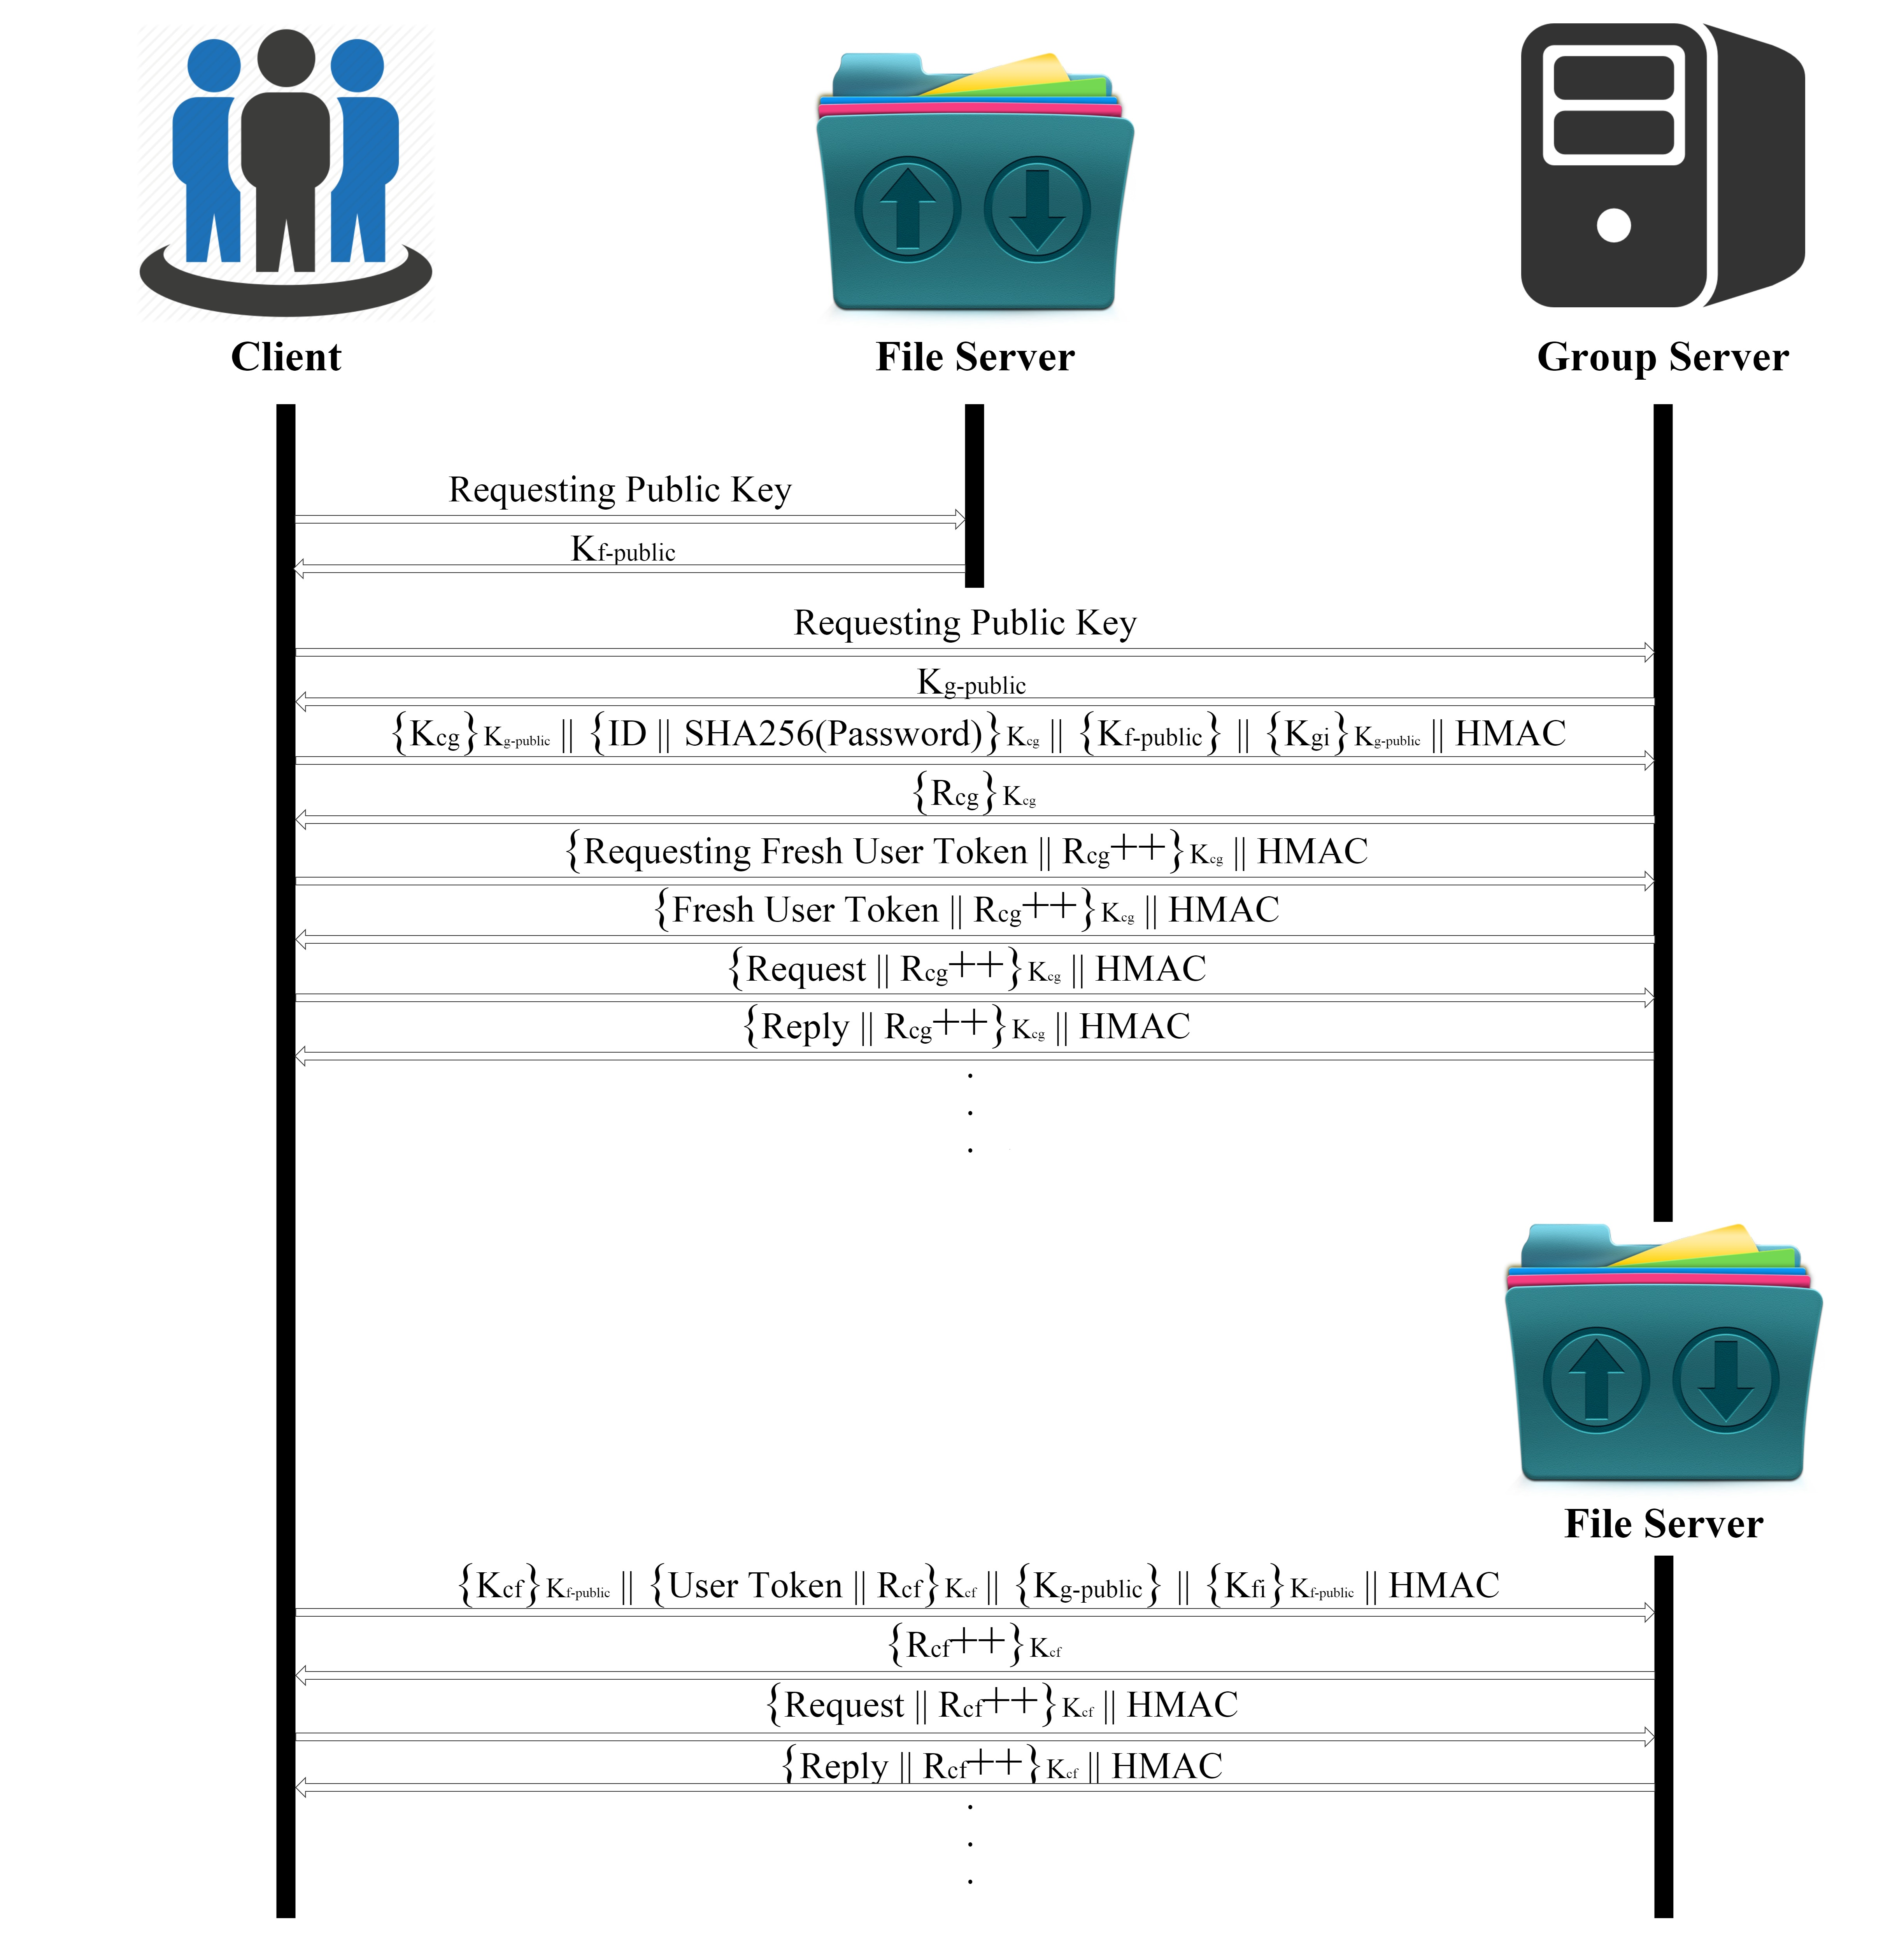
\includegraphics[scale=0.1]{Protocols}
\resheading{T5 Message Reorder, Replay, or Modification}
\vspace{0.1in}
\begin{itemize}[noitemsep,topsep=0pt,parsep=1pt,partopsep=1pt]
	\item\textbf{Threat Description}
	\begin{flushleft}
		In this phase of the project, attackers are assumed to be active as well, so besides confidentiality ensured in the last phase, integrity also becomes our concern. An active attacker may reorder, modify, or save the cipher texts being transmitted, so both client and server would receive a sequence of messages that are out of order, garbled messages, or a supposedly expired messages.   
	\end{flushleft}
	\item\textbf{Mechanism}
	\\\vspace{0.35in}
	%\centering
		%\begin{tabular}{ccc}
			%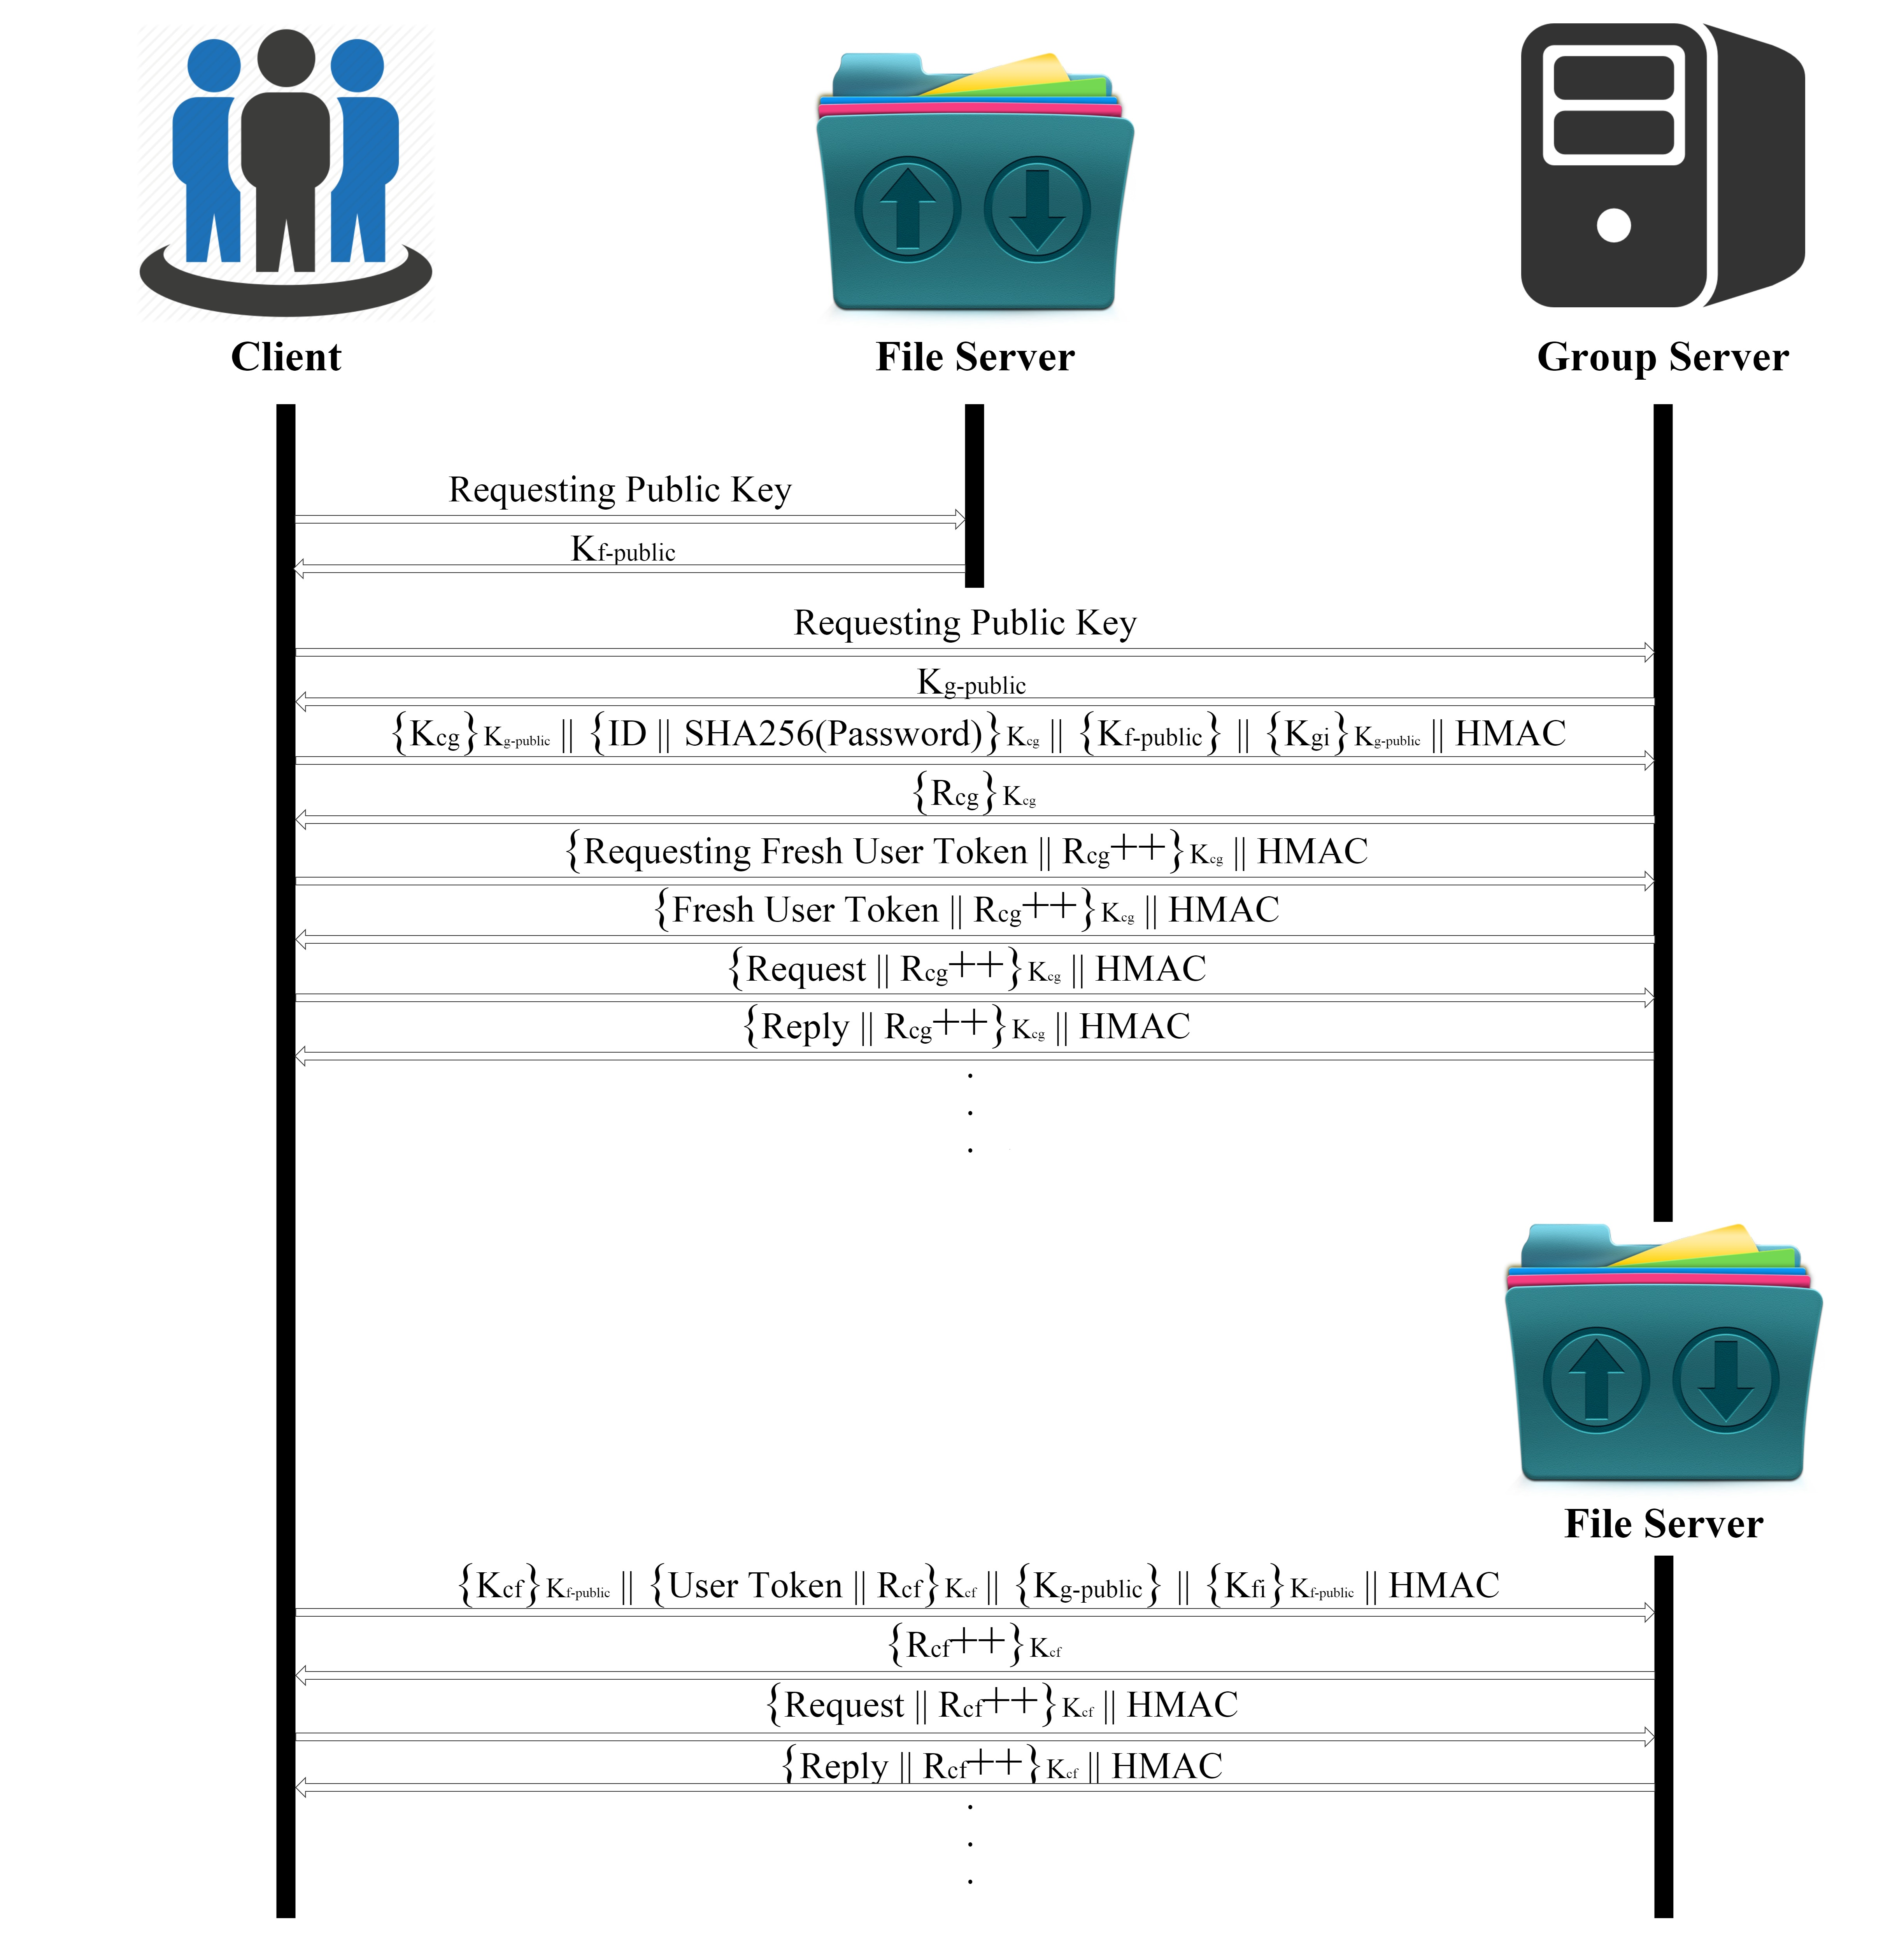
\includegraphics[width=3cm,keepaspectratio]{Protocols}$\,\,\,\,\,$ & 
			%\raisebox{5ex}{%
			%\begin{tabular}{c}
			%	$\,$\\
			%	$\underrightarrow{\quad\,\,\,\,\,\,\,\,\,\,\,\,\,\,\,\,\lbrace R\,||\,msg\rbrace_{key}\,||\,\textrm{HMACSHA256}\left(key,\,R\,||\,msg\right)\,\,\,\,\,\,\,\,\,\,\,\,\,\,\quad}$\\
			%	$\underleftarrow{\quad\,\,\,\,\lbrace R++\,||\,msg\rbrace_{key}\,||\,\textrm{HMACSHA256}\left(key,\,R++\,||\,msg\right)\,\,\quad}$\\
			%	$\underrightarrow{\quad\,\,\,\,\lbrace R++\,||\,msg\rbrace_{key}\,||\,\textrm{HMACSHA256}\left(key,\,R++\,||\,msg\right)\,\,\quad}$\\
			%	$\vdots$\\$\,$\\$\,$\\
			%\end{tabular}} &
			%$\,\,\,\,\,\,\,$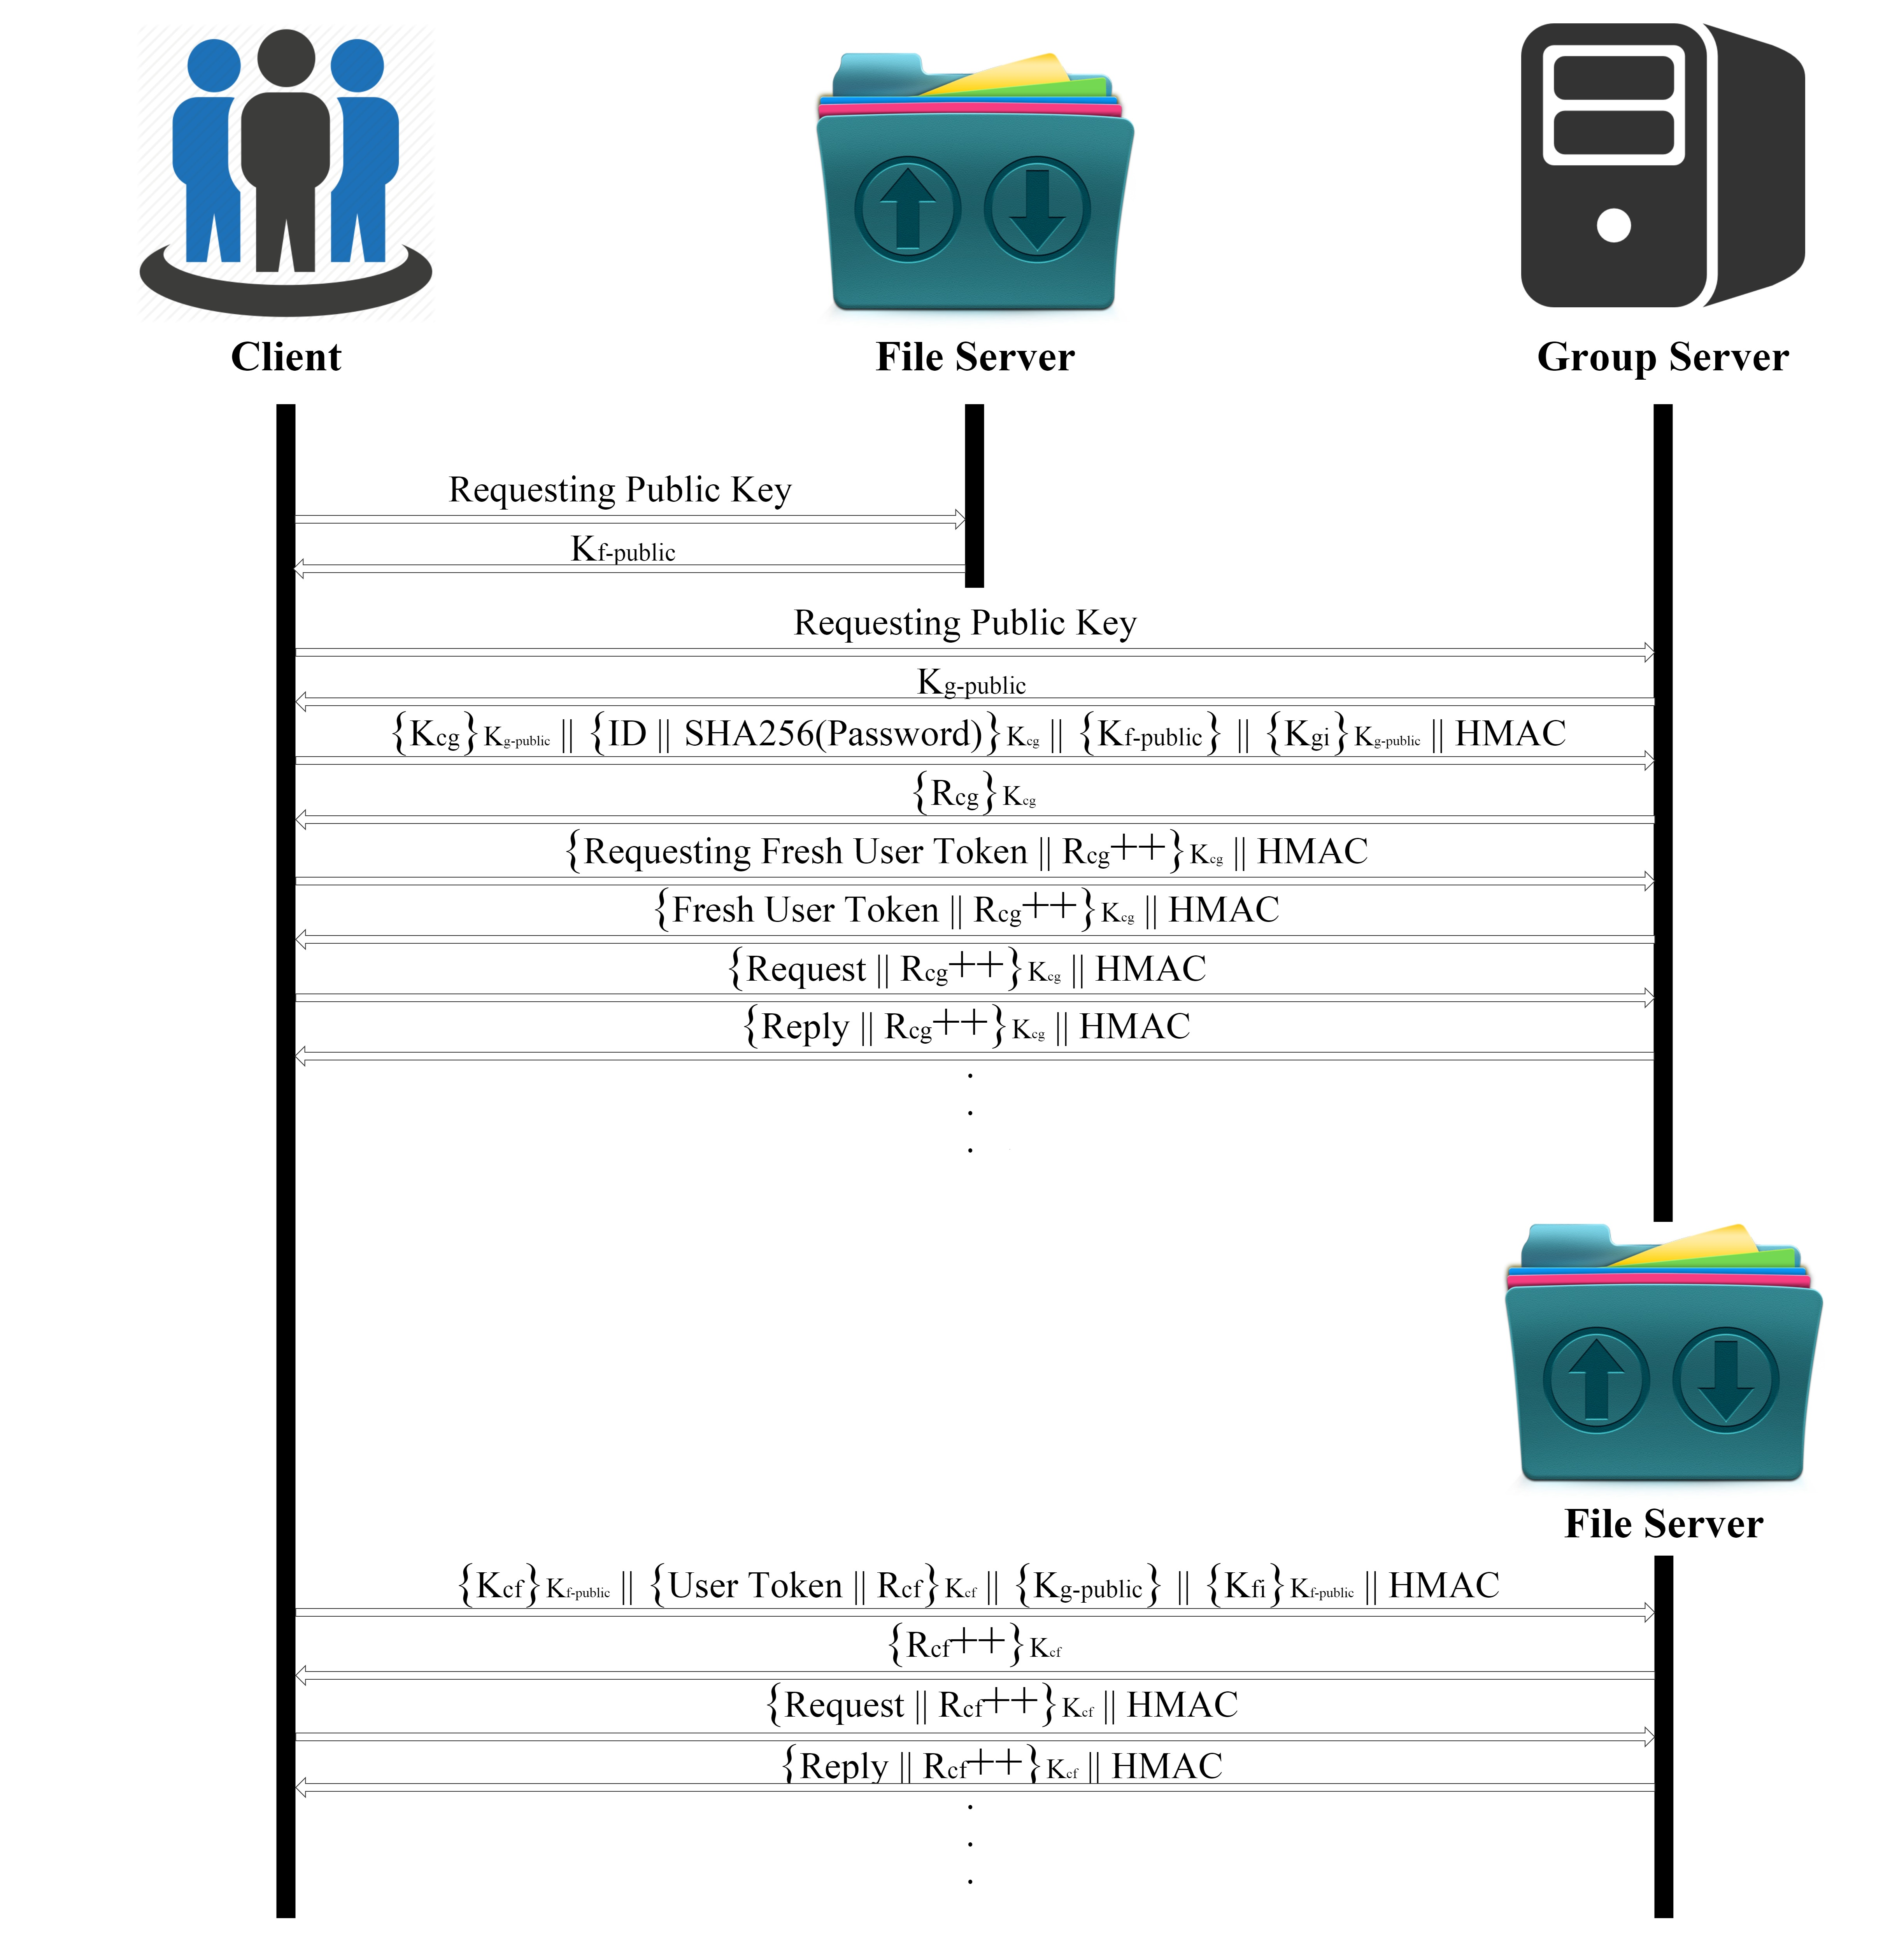
\includegraphics[width=3cm,scale=0.7]{Protocols}
		%\end{tabular}
	\begin{flushleft}
		The above diagram represents a general client-server scenario. The left icon represents clients, and the right icon can represent either the group server or the file server. The $key$ used above might be either a public key or a symmetric key, but for the purpose of T5, we simply represent it as a constant. 
	\end{flushleft}
	\begin{flushleft}
		$R$ is a 64-bit random number chosen by whoever starts the communication, and it will be incremented after every transmission. Both parties will check the decrypted $R$ against the old one so that any reordering attack will be detected immediately. It is also unlikely that any replay attack will succeed. Clearly, an attacker cannot use the intercepted message $c'$ right away because it is computationally infeasible to increment the $R$ within by manipulating the bits of $c'$. To have a successful replay attack, an attacker needs to wait until $R-1$ re-appears, so that $c'$ containing $R$ can be accepted. However, every time $R$ reaches $2^{63}-1$, we will re-randomize $R$, so the chance for an attacker to notice $R-1$ will be either $0$ (re-randomized to $R'>R-1$) or negligibly small. HMAC being used protects message from modification, and we choose SHA-family because the MD-family has been broken in 2008. An attacker may modify cipher text, HMAC, or both, but it is computationally infeasible for him/her to have a meaningful and matched $<\textrm{cipher\_text},\,\textrm{HMAC}>$ pair.
	\end{flushleft}
	%\item\textbf{Correctness/Security}
	%\begin{flushleft}
	 %The shared symmetric session key $K_{cg}$ that both client and server agree upon ensured the correctness of message being transmitting. RSA encryption/decryption used during the initial key exchange secures the later communication for it prevents any third party from knowing $K_{cg}$.    
	%\end{flushleft}
\end{itemize}
    $\,$\\
\resheading{T7 Token Theft}
\vspace{0.1in}
\begin{itemize}[noitemsep,topsep=0pt,parsep=1pt,partopsep=1pt]
	\item\textbf{Threat Description}
	\begin{flushleft}
		If an user token is stolen, then whoever steals it now gain all permissions this token grants -- confidential files shared in the group would now be exposed to the theft, deleted without owner being aware of, or downloaded in secret.
	\end{flushleft}
	\newpage
	\item\textbf{Mechanism}
	\begin{flushleft}
		A stolen token would be useless if it can only reach the theft file server containing no actual files. Since the IP address and the port number uniquely determine a file server, we add an extra filed for token to remember the file server it is communicating with. This new filed will store SHA256$\left(\textrm{IP}\,||\,\textrm{Port\#}\right)$. When an user connects to a theft file server determined by $\textrm{IP}'$ and $\textrm{Port\#}'$, its new field will store SHA256$\left(\textrm{IP}'\,||\,\textrm{Port\#}'\right)$. Theft trying to exploit the stolen token will fail if we force every file server to check the new filed before processing any request. As stated in T2, the group server signs the token before issuance, so the theft will not be able to modify the new filed of the stolen token.
	\end{flushleft}
	%$\,\,\,\,\,\,\,\,\,\,\,\,\,\,\,\,\,\,\,\,\,\,\,\,\,\,$
	%\setlength{\tabcolsep}{10pt}
	%\begin{tabular}{ccc}
	%	
\includegraphics[width=3cm,keepaspectratio]{c} & 
	%	\raisebox{5ex}{%
	%		\begin{tabular}{c}
	%			$\underrightarrow{\quad\,\,\,\,\,\,\,\,\,\,\,\,\,\,\,\,\,\,\,\,\,\,\,\,\,\,\,\,1.\left\lbrace R\,||\,K_{cf}\right\rbrace_{K_{fs}}\,\,\,\,\,\,\,\,\,\,\,\,\,\,\,\,\,\,\,\,\,\,\,\,\,\,\,\,\quad}$\\
	%			$\underleftarrow{\quad\,\,\,\,\,\,\,\,\,\,\,\,\,\,\,\,\,\,\,\,\,\,\,\,\,\,\,\,\,\,\,2.\left\lbrace R-1\right\rbrace_{K_{cf}}\,\,\,\,\,\,\,\,\,\,\,\,\,\,\,\,\,\,\,\,\,\,\,\,\,\,\,\,\,\,\,\quad}$\\
	%			$\underrightarrow{\,\,\,\,\,\,\,\,\,\,\,\,\,\,\,\,\,\,\,\,\,\,\,\quad3.\left\lbrace\textrm{user\_token}\right\rbrace_{K_{cf}}\,\,\,\,\,\,\,\,\,\,\,\,\,\,\,\,\,\,\,\,\,\,\,\,\,\,\quad}$\\
	%			$\,$\\$\,$\\			
	%		\end{tabular}} &
	%		
\includegraphics[width=3cm,scale=1.1]{f}
	%	\end{tabular}
	%\begin{flushleft}
	%	The 
	%\end{flushleft}
		%\item\textbf{Correctness/Security}
		%\begin{flushleft}
		%	 The correctness of the token verification relies mainly on the signature signed by the group server that is assumed trustworthy and will not be compromised. The correct communication between file client and file server depends on the shared key $K_{fs}$ that is exchanged in a RSA secured manner just as the case in the last section.   
		%\end{flushleft}
	\end{itemize}
\end{document}
